\section{Przegląd komercyjnych rozwiązań TRNG}

Współczesne systemy kryptograficzne oraz aplikacje wymagają generowania liczb losowych, które muszą charakteryzować się wysoką jakością i odpornością na przewidywalność. Najlepiej spełniają do generatory liczb losowych oparte na fizycznych zjawiskach, zwane TRNG (True Random Number Generator). TRNG są szczególnie istotne w kontekście aplikacji wymagających silnej ochrony danych, takich jak systemy kryptograficzne, podpisy cyfrowe, oraz w generowaniu kluczy szyfrujących.

\subsection{Rozwiązania sprzętowe}

Wśród komercyjnych rozwiązań sprzętowych, wiodącymi producentami są firmy takie jak \textbf{ID Quantique}, \textbf{Microchip Technology} i \textbf{Semtech}, które oferują zaawansowane urządzenia bazujące na TRNG. Produkty te zapewniają wysoki poziom bezpieczeństwa i są stosowane w wymagających aplikacjach, takich jak bankowość elektroniczna czy systemy wojskowe.

\begin{itemize}
    \item \textbf{ID Quantique} jest jednym z liderów w dziedzinie generatorów liczb losowych opartych na technologii fotoniki. Firma oferuje urządzenia, które wykorzystują detekcję fotonów w celu generowania liczb losowych. Dzięki temu rozwiązania ID Quantique charakteryzują się bardzo wysoką jakością losowości, a jednocześnie są odporne na ataki związane z analizą i przewidywaniem generowanych liczb.

    \item \textbf{Microchip Technology} w swojej ofercie posiada różne moduły TRNG, w tym układy scalone, które generują liczby losowe na podstawie fluktuacji szumów termicznych. Produkty te znajdują zastosowanie w szerokim zakresie aplikacji, od urządzeń mobilnych po systemy wbudowane.

    \item \textbf{Semtech} natomiast oferuje rozwiązania, które wykorzystują zjawiska losowe zachodzące w obwodach analogowych do generowania liczb losowych. Firma ta jest jednym z głównych dostawców układów TRNG, które znajdują szerokie zastosowanie w urządzeniach IoT oraz w systemach komunikacji bezprzewodowej.
\end{itemize}

\subsection{Generatory TRNG w chmurze}

W ostatnich latach pojawiły się także rozwiązania chmurowe, które umożliwiają generowanie liczb losowych w czasie rzeczywistym bez potrzeby posiadania własnego sprzętu. Przykładem takiego rozwiązania jest \textbf{Cloudflare} – firma specjalizująca się w dostarczaniu usług związanych z bezpieczeństwem sieciowym. Na swoim blogu Cloudflare przedstawia zaawansowane metody generowania liczb losowych, które są wykorzystywane w ich systemach.
Cloudflare korzysta z technologii opartych na zjawiskach fizycznych, takich jak "Entropy Wall", czyli seed'owanie PRNG za pomocą danych pochodzących z kamery, ze zdjęć ściany lamp lawowych*,
nieprzewidywalnego fizycznie trójstopniowego wahadła, rozpadu radioaktywnego Uranu oraz procesów związane z tzw. "chaosem kwantowym".
Tego typu rozwiązania pozwalają na szybkie i bezpieczne generowanie liczb losowych w skali globalnej, zapewniając jednocześnie wysoki poziom ochrony przed atakami.

*LavaRand pozostaje dzisiaj jedynie dodatkowym zabezpieczeniem firmy, na wypadek gdyby ich konwencjonalne źródła entropii okazały się niewystarczające, jednak wciąż pozostaje inspirującym przykładem do szukania losowości wszędzie wokół nas.

% rescale?
\begin{figure}[H]
    \centering
    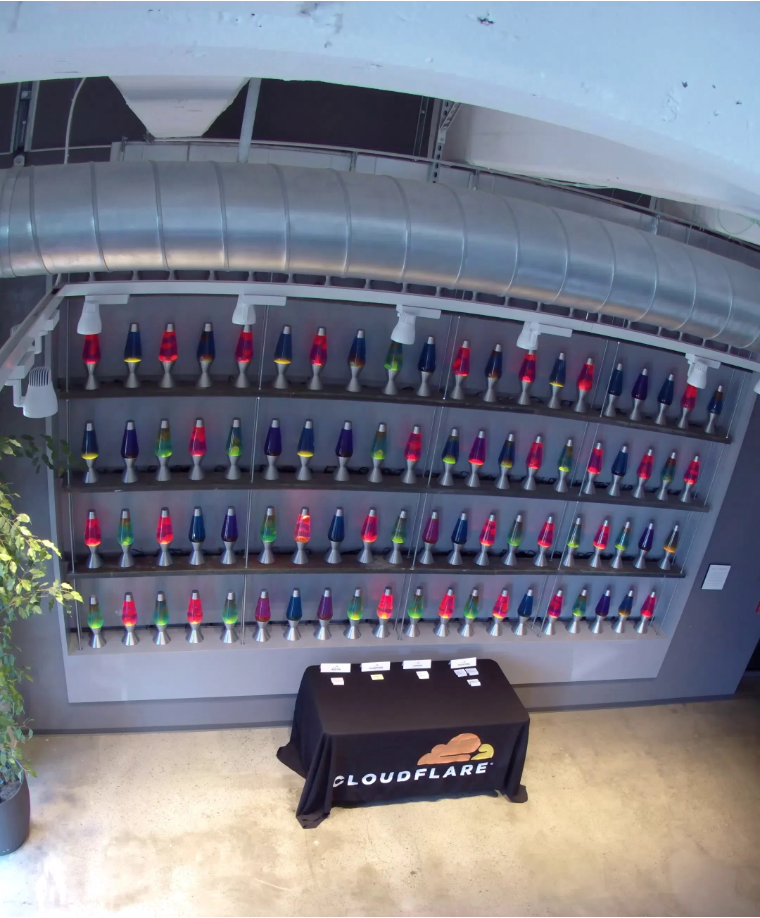
\includegraphics[width=0.4\linewidth]{chapters/02-teoria/figures/lavarandCamera}
    \caption{Widok z kamery w biurze Cloudflare}
    \label{fig:lavarand}
\end{figure}
Źródło: https://blog.cloudflare.com/lavarand-in-production-the-nitty-gritty-technical-details/
TODO - dodać do bibtex'a ;)

Firma ta oferuje użytkownikom dostęp do generatora liczb losowych w chmurze, który jest wykorzystywany
m.in. do tworzenia kluczy kryptograficznych oraz w innych zastosowaniach wymagających silnych zabezpieczeń.
Dzięki wykorzystaniu globalnej infrastruktury Cloudflare generowane liczby losowe są
szeroko dostępne i charakteryzują się dużą niezawodnością oraz odpornością na ataki.


        -----TODO---- \\
    Zrobić mniej poszatkowane \\
    idk kto to zrobi najlepiej, ale w wolnej chwili zerknijcie tu proszę \\
    I TAK ZOSTAWIAM TO W PDF, ŻEBYŚCIE PRZEGLĄDAJĄC NA TO TRAFILI! \\


\section{Wady dostępnych rozwiązań TRNG}

Mimo że Generatory Liczb Losowych Oparte na Zjawiskach Fizycznych (TRNG) oferują wysoki poziom bezpieczeństwa i losowości, istnieje kilka istotnych wad i ograniczeń związanych z ich implementacją i użytkowaniem. Wśród głównych problemów, które mogą wpływać na wydajność oraz niezawodność TRNG, wyróżnia się następujące aspekty:

\subsection{Wydajność i szybkość generowania liczb losowych}

Wydajność TRNG jest często niższa niż w przypadku Generujących Liczby Losowe Oparte na Algorytmach (PRNG). Generowanie liczb losowych za pomocą zjawisk fizycznych, takich jak szum termiczny czy fluktuacje kwantowe, może być procesem czasochłonnym, szczególnie w systemach wymagających dużych ilości losowych liczb w krótkim czasie. W wyniku tego, TRNG mogą nie spełniać wymagań wydajnościowych w aplikacjach o dużym zapotrzebowaniu na losowość, takich jak systemy kryptograficzne o bardzo wysokiej częstotliwości operacji.

\subsection{Koszty implementacji}

Urządzenia TRNG, zwłaszcza te oparte na zaawansowanych technologiach, takich jak fotonika kwantowa czy detekcja szumów kwantowych, mogą wiązać się z wysokimi kosztami produkcji oraz utrzymania. Z tego powodu, TRNG są często droższe w porównaniu do bardziej ekonomicznych rozwiązań opartych na algorytmach deterministycznych (PRNG), które wystarczają do wielu zastosowań, gdzie wysoka jakość losowości nie jest kluczowym wymaganiem.

\subsection{Stabilność i jakość generowanych liczb losowych}

Choć TRNG są uznawane za bezpieczne, ich jakość może być wpływana przez różne czynniki zewnętrzne, takie jak temperatura, zakłócenia elektromagnetyczne czy inne zmiany środowiskowe. W wyniku tego, generowane liczby losowe mogą wykazywać pewne niskiej jakości właściwości, co wymaga zastosowania dodatkowych mechanizmów, takich jak procesy post-przetwarzania, aby zapewnić ich odpowiednią losowość. Nawet małe zakłócenia w systemie mogą prowadzić do wzorców, które mogą zostać wykorzystane w atakach kryptograficznych.

\subsection{Skomplikowana kalibracja i konserwacja}

Urządzenia TRNG, szczególnie te, które wykorzystują skomplikowane zjawiska fizyczne, wymagają starannej kalibracji i ciągłego monitorowania, aby zapewnić ich prawidłowe funkcjonowanie. W wielu przypadkach konieczne jest stosowanie systemów nadzoru, które monitorują jakość generowanych liczb losowych w czasie rzeczywistym. Ponadto, wymogi dotyczące utrzymania odpowiednich warunków pracy, takich jak stabilna temperatura czy brak zakłóceń elektromagnetycznych, mogą stanowić dodatkową przeszkodę w ich szerokim zastosowaniu.

\subsection{Złożoność integracji z istniejącymi systemami}

Integracja TRNG z już działającymi systemami, zwłaszcza w kontekście urządzeń wbudowanych lub systemów o dużych wymaganiach obliczeniowych, może wiązać się z wieloma trudnościami. Często konieczne jest dostosowanie sprzętu lub oprogramowania w celu zapewnienia kompatybilności i pełnej funkcjonalności. Dodatkowo, ze względu na fizyczną naturę tych urządzeń, integracja z innymi komponentami może prowadzić do wzrostu kosztów oraz złożoności całego systemu.

\subsection{Ograniczona dostępność i skalowalność}

Choć rynek TRNG rośnie, nadal jest on stosunkowo niszowy w porównaniu do bardziej powszechnych rozwiązań opartych na PRNG. Ograniczona dostępność wyspecjalizowanych urządzeń TRNG, szczególnie tych, które oferują wysoką jakość generowanych liczb losowych, sprawia, że ich wdrożenie jest trudniejsze, zwłaszcza w przypadkach wymagających masowej produkcji. Ponadto, nie wszystkie rozwiązania są skalowalne, co może być problemem w przypadku aplikacji wymagających elastyczności i łatwego dostosowywania wydajności do rosnących potrzeb.

\subsection{Zagadnienia związane z bezpieczeństwem}

Chociaż TRNG zapewniają wyższy poziom bezpieczeństwa niż PRNG, nie są one całkowicie odporne na ataki. Ataki fizyczne, takie jak manipulacje w obrębie urządzenia lub przechwytywanie sygnałów z jego elementów, mogą prowadzić do kompromitacji jakości liczb losowych. Ponadto, w przypadku rozwiązań opartych na technologii chmurowej, takich jak te oferowane przez Cloudflare, istnieje ryzyko ataków związanych z przechwytywaniem lub manipulowaniem danymi w trakcie transmisji, co może wpływać na bezpieczeństwo generowanych liczb losowych.

\subsection{Podsumowanie wad TRNG}

Chociaż TRNG oferują niezrównaną jakość losowości w porównaniu do rozwiązań opartych na algorytmach, posiadają również szereg wad, które mogą ograniczać ich szerokie zastosowanie. Należy do nich niska wydajność, wysokie koszty implementacji, problemy ze stabilnością generowanych liczb losowych, złożoność integracji z systemami oraz ryzyko związane z bezpieczeństwem. W miarę jak technologia będzie się rozwijać, możliwe jest, że te ograniczenia zostaną przezwyciężone, jednak obecnie stanowią one istotne wyzwanie dla szerokiego przyjęcia TRNG w różnych aplikacjach.

\subsection{Podsumowanie dostępnych na rynku TRNG}